\hypertarget{native_2lwip_2src_2core_2tcp__in_8c}{}\section{/home/ayush/\+R\+I\+O\+T/tests/lwip/bin/pkg/native/lwip/src/core/tcp\+\_\+in.c File Reference}
\label{native_2lwip_2src_2core_2tcp__in_8c}\index{/home/ayush/\+R\+I\+O\+T/tests/lwip/bin/pkg/native/lwip/src/core/tcp\+\_\+in.\+c@{/home/ayush/\+R\+I\+O\+T/tests/lwip/bin/pkg/native/lwip/src/core/tcp\+\_\+in.\+c}}
{\ttfamily \#include \char`\"{}lwip/opt.\+h\char`\"{}}\newline
Include dependency graph for tcp\+\_\+in.\+c\+:
\nopagebreak
\begin{figure}[H]
\begin{center}
\leavevmode
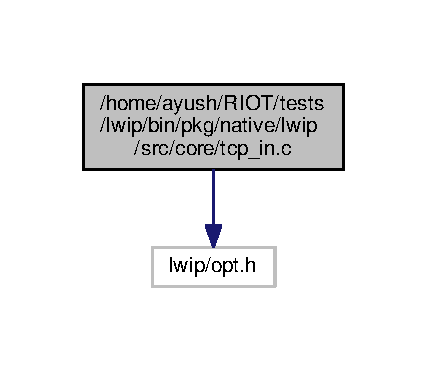
\includegraphics[width=205pt]{native_2lwip_2src_2core_2tcp__in_8c__incl}
\end{center}
\end{figure}


\subsection{Detailed Description}
Transmission Control Protocol, incoming traffic

The input processing functions of the T\+CP layer.

These functions are generally called in the order (ip\+\_\+input() -\/$>$) tcp\+\_\+input() -\/$>$ $\ast$ tcp\+\_\+process() -\/$>$ tcp\+\_\+receive() (-\/$>$ application). 